\documentclass{article}
\usepackage[a4paper, total={6in, 10in}]{geometry}
\usepackage{amsmath}
\usepackage{amssymb}
\usepackage{graphicx}
\usepackage{tcolorbox}

\begin{document}

\Large
\begin{centering} \textbf{Chapter 1: Units, Physical Quantities, and Vectors}

\end{centering}

\section*{Learning Goals}
\large
At the end of this tutorial, you should be able to:
\begin{itemize}
    \item Illustrate vector operations such as addition, subtraction, and scalar multiplication;
    \item Understand and articulate the concept of displacement;
    \item Determine total displacement using vectors.
    
\end{itemize}

\hline \vspace{0.5cm}

\subsection*{1. Drawing Vectors}
In each case below, draw $\vec{C}$ on the figure and find the components $C_x$ and $C_y$.
\newline \vspace{0.5cm}

\noindent a. $\vec{C} = \vec{A} + \vec{B}$
\begin{figure}[h!]
    \centering
    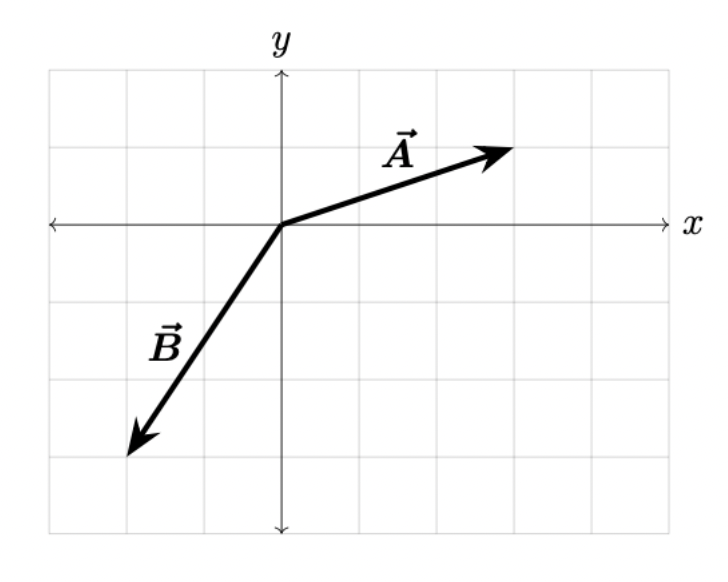
\includegraphics[width=8cm]{case1.png}
\end{figure}

\newpage

\noindent b. $\vec{C} = \vec{A} - \vec{B}$
\begin{figure}[h!]
    \centering
    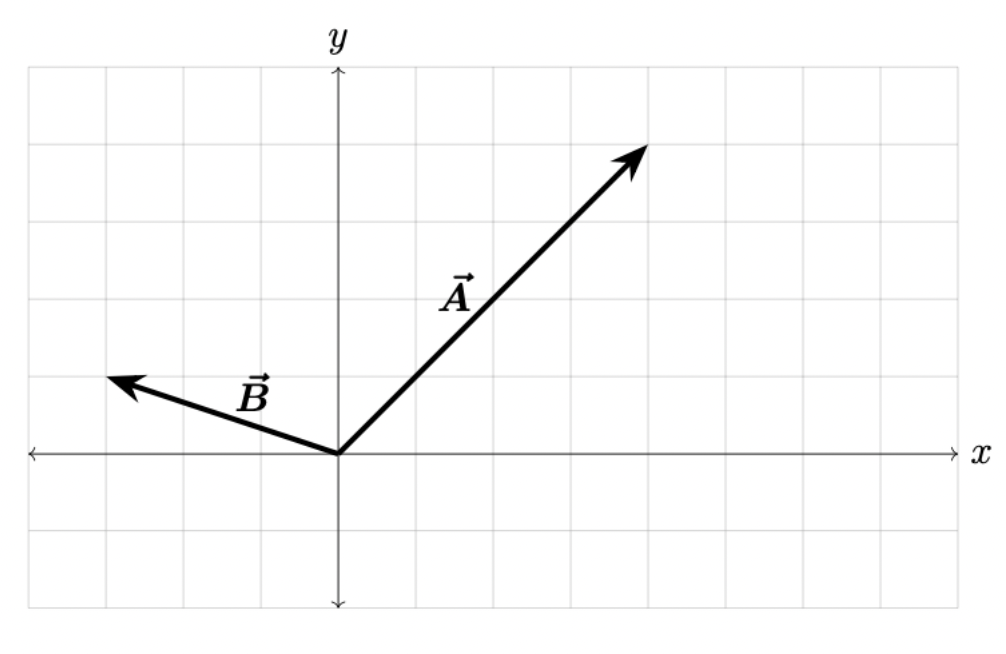
\includegraphics[width=8cm]{case2.png}
\end{figure}

\vspace{4cm}

\noindent c. $\vec{C} = 2\vec{A} - 3\vec{B}$
\begin{figure}[h!]
    \centering
    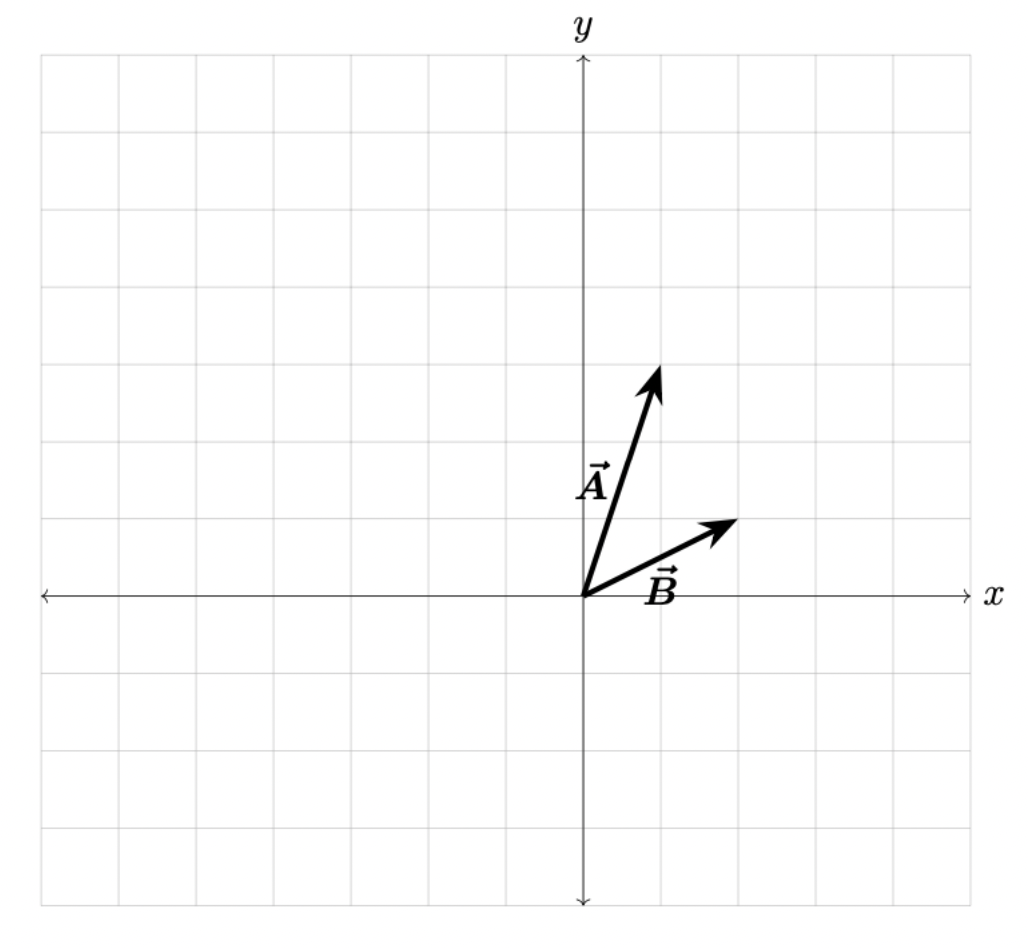
\includegraphics[width=8cm]{case3.png}
\end{figure}

\vspace*{\vfill}
\begin{tcolorbox}[colback=green!5,colframe=green!75!black]
\textbf{STOP -- } Check in with an instructor or another group before moving on.
\end{tcolorbox}

\newpage

\subsection*{2. Travel Between Points}
You travel from point $P$ to point $Q$ in three stages. First, starting at $P$, you travel 7.00 km due east. Then you travel 8.00 km at an angle of 35.0$^\circ$ west of north. Finally, you travel 2.00 km due south, ending at $Q$.
\vspace{0.5cm}

\noindent a. Draw a picture of the scenario above. Label points $P$ and $Q$ in your drawing, as well as each stage of travel. 
\vspace{5cm}

\noindent b. In words, explain the concept of displacement. What is the difference between distance and displacement?

\vspace{5cm}

\noindent c. What is the displacement from $P$ to $Q$? (\textit{Hint: How can you use the vectors you drew in part a to find the displacement?})
\vspace*{\vfill}
\begin{tcolorbox}[colback=green!5,colframe=green!75!black]
\textbf{STOP -- } Check in with an instructor or another group before moving on.
\end{tcolorbox}

\newpage

\subsection*{\textbf{Challenge Problem:} Traveling Ants}
Two ants start at the same point. They both return to the hive, but along different paths.
Each ant’s path consists of two stages. Ant #1 first travels 7.00 m in a direction 28.0$^\circ$ east of south and then travels 8.50 m in a direction 58.3$^\circ$ north of east. Ant #2 first travels 5.20 m in a direction 17.9$^\circ$west of north. What is the displacement of ant #2 in the second stage of its trip, ending at the hive? 
\vspace*{\vfill}
\begin{tcolorbox}[colback=green!5,colframe=green!75!black]
\textbf{STOP -- } Check in with an instructor or another group before moving on.
\end{tcolorbox}

\end{document}